\section{Бифур. удв. периода}

\begin{frame}
	\frametitle{Отображение Пуанкаре}

	Введём в пространстве плоскость вдоль направления одного из мультипликаторов. Тогда оставшиеся оставшиеся траектории других будут прижиматься к плоскости.

	Разрежем поток траекторий вблизи этой плоскости некоторой секущей поверхностью. Каждая траектория повторно пересекая эту поверхность ставит в соответствие $x_j \leadsto x_{j+1}$.

	Связь $\vc{x}_{j+1} = f (\vc{x}_j:R)$ называют \textbf{отображением Пуанкаре} (или отображением последования)
	Дискретная о играет роль времени.

\end{frame}

\begin{frame}
	\frametitle{К одномерному случаю}

	Одномерное отображение Пуанкаре дает альтернативный способ определения характера течения вблизи бифуркации. 
	
	\phantom{42}

	Самому периодическому движению отвечает \textbf{неподвижная точка} -- значение $x_j = x_*$, не меняющееся при отображении. Неподвижная точка также может быть устойчивой и нет, в зависимости от $|\mu|$.
\end{frame}

\begin{frame}
	\frametitle{Бифуркация удвоения периода}

	Рассмотрим переход $\mu$ через значение $-1$ в окрестности предельного цикла с периодом $T_0$, вследствие которого возникает новый предельный цикл с периодом $2 T_0$ -- бифуркация удвоения периода.

	\phantom{42}

	Вблизи $x=0$ отображение, описывающее бифуркацию удвоения периода:

	$$x_{j+1} = - [1 + (R - R_1)]x_j + x_j^2 + \beta x_j^3,$$ 
\end{frame}

\begin{frame}
	\frametitle{Путь в возникновение турбулентности}
	Двукратная же итерация того же преобразования приводит к отображению:

$$x_{j+2} = x_j + 2(R-R_1)x_j - 2(1+\beta)x_j^3.$$

При $R>R_1$ точка $x_*=0$ становится неустойчивой.
В этот момент рождается пара устойчивых неподвижных точек $x_*^{(1),(2)} = \pm \left[\frac{R -R_1}{1+\beta}\right]^{1/2}$,
которые и соответствуют устойчивому предельному циклу удвоенного периода.
\end{frame}

\begin{frame}
	\frametitle{Логистическое отображение}
	Простейшим примером отображения Пуанкаре является \textbf{логистическое отображение}.

	\phantom{42}

	В частности модель популяции вида с ограниченными ресурсами принимает такой вид:

	$$ x_{n+1} = \lambda x_n \left( 1 - \frac{x_n}{M}  \right),$$


\end{frame}

\begin{frame}
	\frametitle{Построение}

	Упростим выражение, обозначив за $x$ выражение $x \cdot M$, тогда имеем \textbf{логистического отображение}: 

	$$x_{n+1} = \lambda x_n \left( 1 - x_n  \right).$$

	\begin{figure}
    \centering
    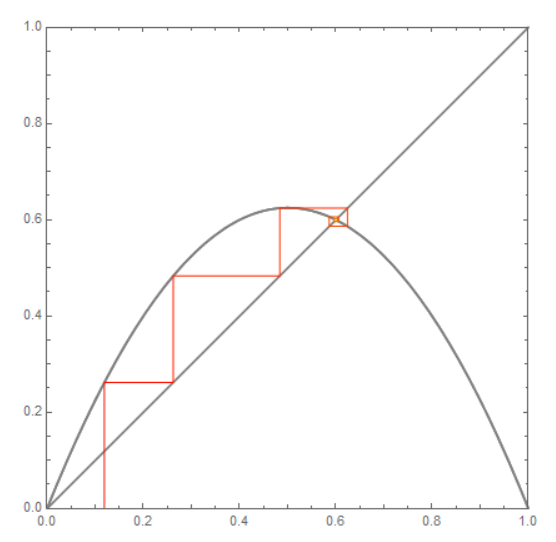
\includegraphics[width=0.24\textwidth]{img/25.png}
    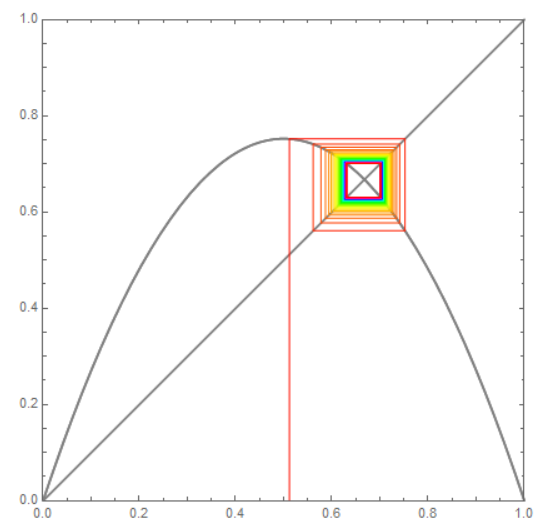
\includegraphics[width=0.24\textwidth]{img/3.png}
    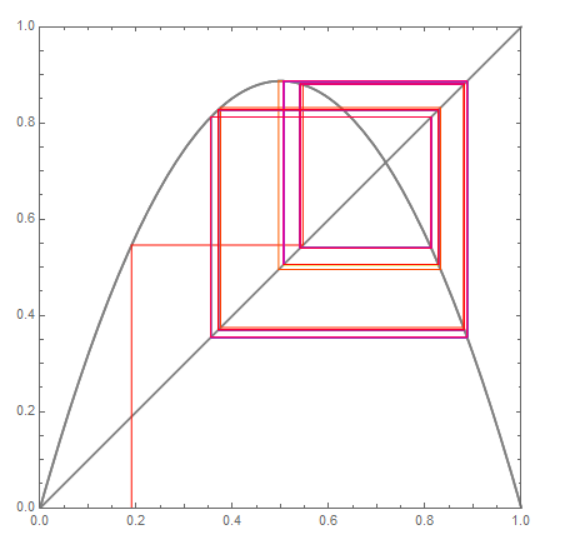
\includegraphics[width=0.24\textwidth]{img/355.png}
    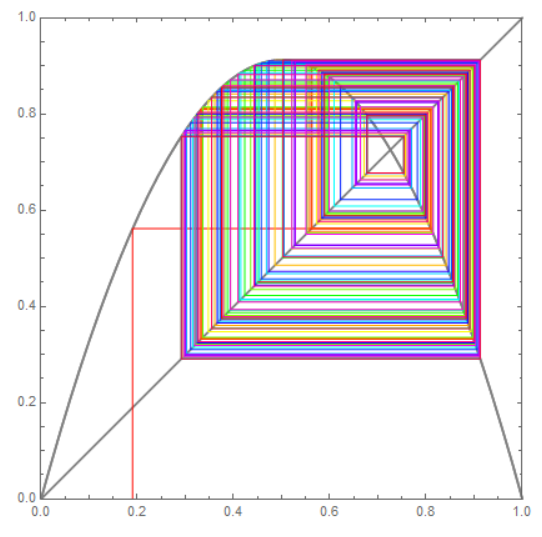
\includegraphics[width=0.24\textwidth]{img/365.png}
    \label{fig:lbl}
\end{figure}
\end{frame}

\begin{frame}
	\frametitle{Интересные значения}

	Для данного отображения в \textit{Python} была рассчитана зависимость показателя Ляпунова от параметра:

	        \centering
        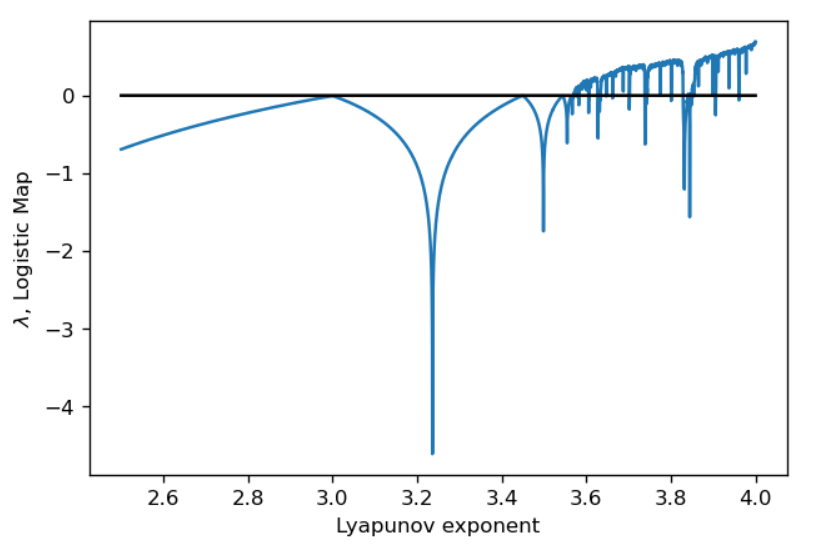
\includegraphics[width=0.6\linewidth]{img/lyap_exp.png}
\end{frame}

\begin{frame}
	\frametitle{Интересные значения}

	Аналогично расчитана зависимость для отображения Гаусса, характеризующееся двумя параметрами $\alpha$ и $\beta$.

\phantom{42}

	        \centering
	    Зависимость $\lambda (\alpha, \beta)$.\\
        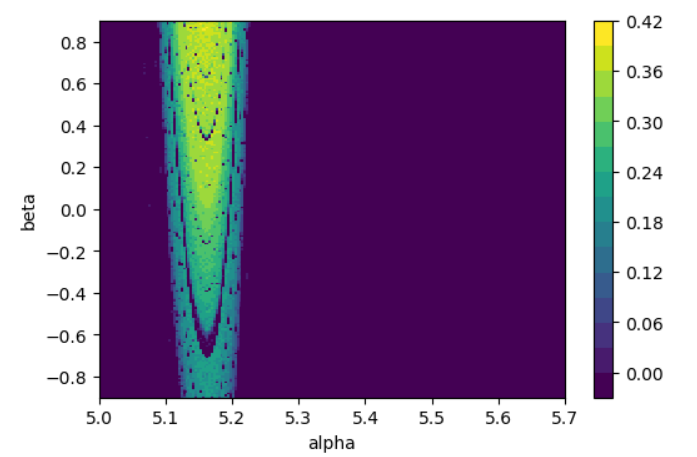
\includegraphics[width=0.6\linewidth]{img/Gauss_map.png}
\end{frame}

\section{Итоги}

\begin{frame}
	\frametitle{Литература}

	\begin{thebibliography}{2}
\addcontentsline{toc}{section}{\bibname}
\bibitem{LL6}
Ландау Л. Д., Лифшиц Е. М., Теоретическая физика. (т. 6) -- Наука. -- ISBN 5-9221-0055-6.
\bibitem{HS}
W. Hirsch, S. Smale, Differential Equations, Dynamical Systems, and an Introduction to Chaos
3rd Edition. -- ISBN: 9780123820112.
\bibitem{Kuz}
С. П. Кузнецов, Динамический хаос (курс лекций). -- М: Физматлит, 2001.
\bibitem{water_wheel}
J. Gleick, Chaos, -- Penguin books, 1987.
\bibitem{LH1}
Rus. J. Nonlin. Dyn., 2012, vol. 8, no. 5, pp. 863–873 (Russian)
\end{thebibliography}
\end{frame}

\begin{frame}
	\begin{itemize}
	\item[$\checkmark$] В итоге в ходе работы была изучена подходы к возникновению турбулентности, изучена теория, относящаяся к ним.
	\item[$\checkmark$] С помощью численного моделирования были рассчитаны и построены решения получившихся систем.
	\item[$\checkmark$] Также решена задача и предпринята попытка экспериментально воссоздать условия зарождения хаотичного движения.
	\item[$\checkmark$] Прочитаны статьи на связанные темы.
	\end{itemize}
\end{frame}

\begin{frame}
	\frametitle{Спасибо за внимание!}
\end{frame}